\scanpage{3}
% crop-candidate: scan 3
\figure{%
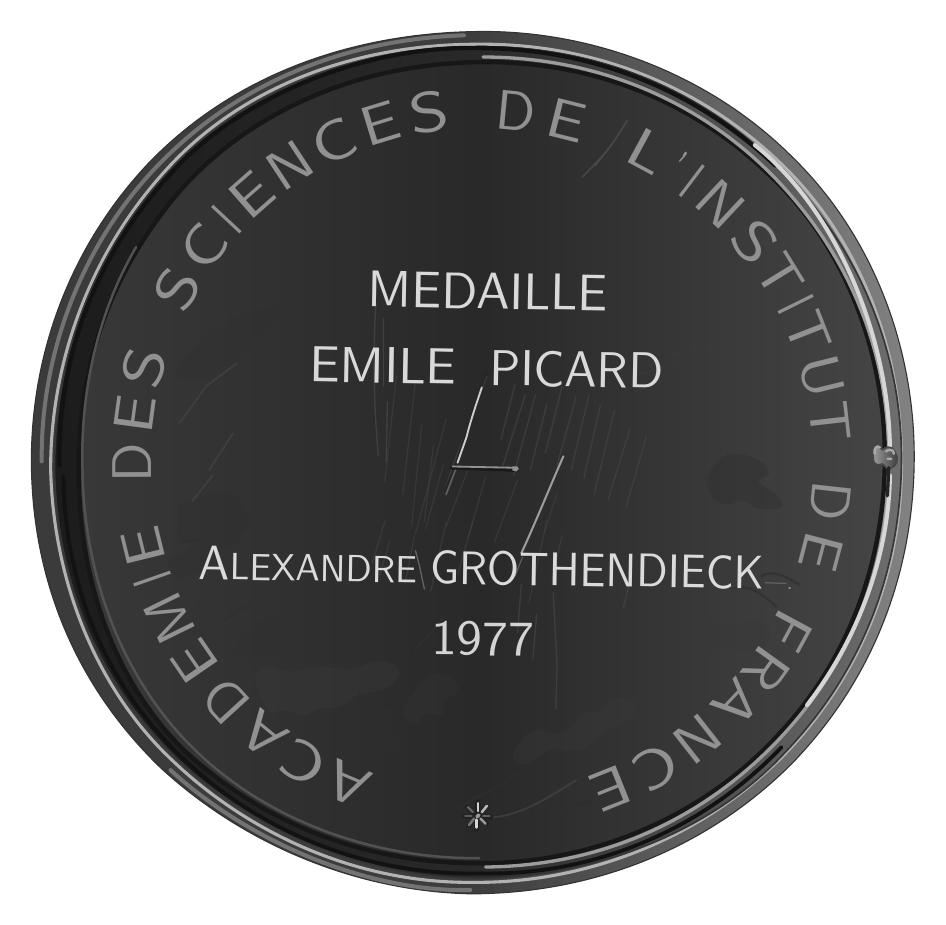
\begin{tikzpicture}[x=0.162mm,y=-0.162mm,line join=round,line cap=round]
  \path[use as bounding box] (65,114) rectangle (763,795);
  % Outer edge, concentric mouldings and inner field.
  \path[shade,left color=black!77,right color=black!49,middle color=black!76,draw=black!80,line width=0.4pt] (419,117) .. controls (508,116) and (600,151) .. (664,215)
      .. controls (728,277) and (760,365) .. (760,450) .. controls (760,542) and (727,626) .. (664,691)
      .. controls (596,759) and (506,793) .. (412,793) .. controls (322,791) and (234,754) .. (169,694)
      .. controls (105,632) and (70,552) .. (68,461) .. controls (66,372) and (98,286) .. (159,221)
      .. controls (226,151) and (319,118) .. (419,117) -- cycle;
  \path[draw=black!55,line width=1.45pt] (76,454) .. controls (75,362) and (113,275) .. (172,217)
      .. controls (233,156) and (316,123) .. (407,120) (412,790)
      .. controls (333,792) and (239,753) .. (177,696);
  \path[draw=black!30,line width=1.12pt] (83,460) .. controls (83,373) and (116,288) .. (174,225)
      .. controls (231,162) and (318,128) .. (413,127) .. controls (508,125) and (593,160) .. (656,221)
      .. controls (717,280) and (750,365) .. (750,453) .. controls (751,538) and (720,620) .. (658,684)
      .. controls (595,748) and (505,785) .. (414,784) .. controls (325,785) and (240,747) .. (179,689)
      .. controls (119,633) and (85,548) .. (83,460);
  \path[shade,left color=black!89,right color=black!57,middle color=black!84,draw=black!79,line width=0.6pt] (418,129) .. controls (507,128) and (591,160) .. (653,223)
      .. controls (716,284) and (750,367) .. (750,451) .. controls (750,541) and (718,621) .. (657,684)
      .. controls (598,747) and (504,781) .. (416,781) .. controls (329,780) and (244,744) .. (184,689)
      .. controls (118,626) and (87,544) .. (86,457) .. controls (87,368) and (118,288) .. (177,225)
      .. controls (238,160) and (328,130) .. (418,129) -- cycle;
  \path[draw=black!93,line width=1.55pt] (90,457) .. controls (88,363) and (125,282) .. (184,221)
      .. controls (236,168) and (328,128) .. (418,130) .. controls (508,130) and (589,163) .. (651,222);
  \path[draw=black!93,line width=1.38pt] (93,466) .. controls (94,555) and (129,634) .. (190,690)
      .. controls (249,745) and (332,779) .. (420,777) .. controls (507,779) and (593,744) .. (656,678);
  \path[shade,left color=black!78,right color=black!73,middle color=black!84,draw=black!91,line width=1.6pt] (420,141) .. controls (504,140) and (584,169) .. (647,230)
      .. controls (707,286) and (737,370) .. (737,451) .. controls (737,533) and (708,613) .. (649,673)
      .. controls (589,736) and (502,770) .. (418,769) .. controls (330,769) and (251,739) .. (187,680)
      .. controls (132,625) and (104,545) .. (105,456) .. controls (105,376) and (132,302) .. (186,240)
      .. controls (243,177) and (328,142) .. (420,141) -- cycle;
  \path[draw=black!39,line width=1.2pt] (422,137) .. controls (511,137) and (591,171) .. (649,230)
      .. controls (705,287) and (739,361) .. (740,447) .. controls (741,539) and (711,612) .. (652,674)
      .. controls (591,737) and (513,771) .. (424,772);
  \path[draw=black!16,line width=1.45pt] (635,206) .. controls (699,257) and (740,356) .. (741,444) (741,465)
      .. controls (740,529) and (716,593) .. (676,645);
  \path[draw=black!68,line width=0.9pt] (150,286) .. controls (120,337) and (106,400) .. (108,461)
      .. controls (109,542) and (138,621) .. (191,675) .. controls (249,735) and (336,766) .. (419,765);
  \begin{scope}
  \clip (420,141) .. controls (504,140) and (584,169) .. (647,230)
      .. controls (707,286) and (737,370) .. (737,451) .. controls (737,533) and (708,613) .. (649,673)
      .. controls (589,736) and (502,770) .. (418,769) .. controls (330,769) and (251,739) .. (187,680)
      .. controls (132,625) and (104,545) .. (105,456) .. controls (105,376) and (132,302) .. (186,240)
      .. controls (243,177) and (328,142) .. (420,141) -- cycle;
  % Worn areas of the field and the principal visible scores.
  \path[opacity=0.3,fill=black!81] (185,375) .. controls (213,347) and (230,334) .. (266,332)
      .. controls (248,349) and (239,369) .. (224,376) .. controls (213,381) and (202,393) .. (191,392)
      -- (181,386) -- cycle;
  \path[opacity=0.3,fill=black!82] (183,488) .. controls (205,480) and (219,475) .. (229,481) -- (241,501) -- (229,518) -- (210,527)
      -- (203,540) -- (182,546) -- (174,534) -- (194,519) -- (182,515) -- cycle;
  \path[opacity=0.3,fill=black!80] (201,552) .. controls (227,540) and (240,543) .. (250,536) -- (273,539) -- (270,553) -- (255,564)
      -- (237,573) -- (223,577) -- (207,592) -- (192,587) -- cycle;
  \path[opacity=0.3,fill=black!81] (235,586) .. controls (264,569) and (289,562) .. (319,566) -- (331,578) -- (303,591) -- (285,592)
      -- (265,606) -- (251,604) -- (238,612) -- (227,602) -- cycle;
  \path[opacity=0.3,fill=black!76] (245.85,633.75) .. controls (241.95,623.25) and (242.85,617.40) .. (250.45,615.80)
      .. controls (256.15,614.60) and (260.95,614.90) .. (266.15,617.30)
      .. controls (270.05,619.10) and (275.30,619.10) .. (284.10,616.70)
      .. controls (290.70,614.90) and (297.75,614.60) .. (307.75,616.20)
      .. controls (315.25,617.40) and (322.30,616.50) .. (331.10,612.50)
      .. controls (337.70,609.50) and (343.85,609.35) .. (351.45,612.95)
      .. controls (357.15,615.65) and (358.05,619.55) .. (352.85,626.35)
      .. controls (348.95,631.45) and (343.25,634.30) .. (333.25,635.10)
      .. controls (325.75,635.70) and (320.20,637.80) .. (315.40,642.60)
      .. controls (311.80,646.20) and (307.00,647.85) .. (299.00,647.45)
      .. controls (293.00,647.15) and (289.10,648.20) .. (286.70,651.40)
      .. controls (284.90,653.80) and (281.30,653.95) .. (274.10,651.15)
      .. controls (268.70,649.05) and (264.05,648.75) .. (258.85,650.75)
      .. controls (254.95,652.25) and (251.05,647.75) .. (245.85,633.75) -- cycle;
  \path[opacity=0.3,fill=black!81] (289.80,668.05) .. controls (282.60,665.35) and (283.20,660.85) .. (294.40,652.45)
      .. controls (302.80,646.15) and (309.85,644.35) .. (317.45,647.95)
      .. controls (323.15,650.65) and (328.40,650.65) .. (334.80,647.05)
      .. controls (339.60,644.35) and (343.95,644.50) .. (349.15,648.50)
      .. controls (353.05,651.50) and (354.25,654.80) .. (352.25,659.60)
      .. controls (350.75,663.20) and (352.25,666.50) .. (358.25,670.50)
      .. controls (362.75,673.50) and (363.20,676.65) .. (358.40,681.05)
      .. controls (354.80,684.35) and (349.25,684.35) .. (339.25,679.95)
      .. controls (331.75,676.65) and (325.75,676.50) .. (319.75,680.50)
      .. controls (315.25,683.50) and (311.50,683.20) .. (307.50,678.40)
      .. controls (304.50,674.80) and (299.40,671.65) .. (289.80,668.05) -- cycle;
  \path[opacity=0.3,fill=black!79] (361.75,656.40) .. controls (357.25,652.80) and (358.75,646.05) .. (368.75,632.85)
      .. controls (376.25,622.95) and (383.00,618.90) .. (391.00,621.30)
      .. controls (397.00,623.10) and (400.60,625.65) .. (402.20,630.05)
      .. controls (403.40,633.35) and (401.90,636.05) .. (396.30,638.85)
      .. controls (392.10,640.95) and (390.30,643.80) .. (391.10,648.60)
      .. controls (391.70,652.20) and (389.45,653.55) .. (382.65,652.35)
      .. controls (377.55,651.45) and (374.25,652.80) .. (372.25,657.60)
      .. controls (370.75,661.20) and (367.75,661.20) .. (361.75,656.40) -- cycle;
  \path[opacity=0.3,fill=black!77] (447.85,689.50) .. controls (443.95,686.50) and (444.85,681.55) .. (452.45,672.35)
      .. controls (458.15,665.45) and (464.75,663.20) .. (474.75,666.40)
      .. controls (482.25,668.80) and (488.25,666.85) .. (494.25,658.45)
      .. controls (498.75,652.15) and (503.10,649.30) .. (508.70,650.10)
      .. controls (512.90,650.70) and (516.35,648.90) .. (519.95,643.30)
      .. controls (522.65,639.10) and (527.00,637.90) .. (535.00,640.30)
      .. controls (541.00,642.10) and (543.10,645.10) .. (540.70,650.70)
      .. controls (538.90,654.90) and (534.55,658.50) .. (525.35,662.50)
      .. controls (518.45,665.50) and (512.45,669.40) .. (505.65,675.80)
      .. controls (500.55,680.60) and (494.40,682.10) .. (484.80,679.70)
      .. controls (477.60,677.90) and (471.15,679.70) .. (463.55,686.90)
      .. controls (457.85,692.30) and (453.05,693.50) .. (447.85,689.50) -- cycle;
  \path[opacity=0.3,fill=black!78] (566.20,601.70) .. controls (561.40,599.90) and (562.15,596.45) .. (570.55,589.65)
      .. controls (576.85,584.55) and (583.30,581.70) .. (592.10,580.90)
      .. controls (598.70,580.30) and (603.50,580.60) .. (607.50,582.20)
      .. controls (610.50,583.40) and (615.00,582.95) .. (623.00,580.15)
      .. controls (629.00,578.05) and (634.55,577.90) .. (641.35,580.30)
      .. controls (646.45,582.10) and (648.55,585.40) .. (647.35,591.80)
      .. controls (646.45,596.60) and (643.00,599.75) .. (635.00,601.75)
      .. controls (629.00,603.25) and (623.00,602.95) .. (615.00,600.15)
      .. controls (609.00,598.05) and (603.45,598.65) .. (596.65,603.05)
      .. controls (591.55,606.35) and (586.90,607.55) .. (581.30,606.35)
      .. controls (577.10,605.45) and (572.60,604.10) .. (566.20,601.70) -- cycle;
  \path[opacity=0.3,fill=black!83] (598.75,466.00) .. controls (600.25,460.00) and (603.25,455.35) .. (609.25,450.95)
      .. controls (613.75,447.65) and (619.45,446.90) .. (628.65,449.30)
      .. controls (635.55,451.10) and (640.50,453.95) .. (644.50,459.15)
      .. controls (647.50,463.05) and (646.75,465.60) .. (640.75,467.20)
      .. controls (636.25,468.40) and (636.70,470.50) .. (643.90,474.50)
      .. controls (649.30,477.50) and (653.20,480.80) .. (656.40,485.60)
      .. controls (658.80,489.20) and (656.40,491.15) .. (646.80,491.55)
      .. controls (639.60,491.85) and (634.50,490.65) .. (630.50,487.05)
      .. controls (627.50,484.35) and (623.75,484.05) .. (617.75,486.85)
      .. controls (613.25,488.95) and (608.75,488.05) .. (602.75,482.85)
      .. controls (598.25,478.95) and (596.75,474.00) .. (598.75,466.00) -- cycle;
  \path[opacity=0.67,draw=black!71,line width=0.48pt] (338,331) .. controls (335,375) and (337,419) .. (340,450) (344,342) -- (344,395) (347,407)
      -- (346,454);
  \path[opacity=0.67,draw=black!76,line width=0.48pt] (354,387) -- (345,470) (369,391) -- (359,480) (374,425) -- (366,504) (383,442) -- (376,501);
  \path[opacity=0.67,draw=black!73,line width=0.47pt] (425,387) -- (400,453) -- (391,479) (447,394) -- (436,437) (455,402) -- (436,462) (463,402)
      -- (446,465) (472,409) -- (459,461);
  \path[opacity=0.67,draw=black!73,line width=0.45pt] (484,395) -- (471,447) (495,403) -- (480,457) (505,402) -- (491,461) (514,410) -- (501,467)
      (525,414) -- (509,480) (537,429) -- (520,484) (550,435) -- (534,490);
  \path[opacity=0.67,draw=black!75,line width=0.4pt] (393,421) -- (369,511) (391,456) -- (377,507) (410,461) -- (393,505) (424,466) -- (410,515)
      (449,469) -- (431,517) (480,479) -- (470,510);
  \path[opacity=0.67,draw=black!75,line width=0.45pt] (345,501) -- (335,534) (349,516) -- (341,543) (368,513) -- (361,550) (393,502) -- (381,556)
      (414,501) -- (402,543) (472,500) -- (458,565) (484,512) -- (476,547);
  \path[opacity=0.67,draw=black!73,line width=0.5pt] (477,557) -- (480,614) -- (479,648) (452,550) -- (449,588) (464,574) -- (461,609) (537,548)
      -- (532,569);
  \path[opacity=0.67,draw=black!77,line width=0.47pt] (551,379) -- (575,369) -- (604,365) (544,386) -- (582,374) (541,399) -- (575,386);
  \path[opacity=0.67,draw=black!73,line width=0.65pt] (184,424) -- (205,395) -- (229,377) (207,461) -- (226,432) (194,485) -- (210,465) (430,733)
      .. controls (455,731) and (478,714) .. (495,704);
  \path[opacity=0.67,draw=black!68,line width=0.61pt] (535,187) -- (524,204) -- (510,222) (519,211) -- (500,231);
  \path[opacity=0.67,draw=black!82,line width=0.86pt] (402,726) .. controls (418,716) and (451,701) .. (463,688) (452,748) -- (481,731) -- (507,719);
  \path[opacity=0.67,draw=black!81,line width=0.87pt] (184,518) -- (201,514) -- (211,509) (219,578) -- (240,566) (369,602) -- (390,577) (617,554)
      .. controls (629,549) and (641,558) .. (652,568) (640,544)
      .. controls (648,539) and (658,543) .. (670,551);
  \path[draw=black!85,line width=0.95pt] (425,384) .. controls (420,393) and (416,411) .. (410,427) -- (401,456) -- (392,478);
  \path[draw=black!20,line width=0.69pt] (421,396) .. controls (416,411) and (412,423) .. (409,435) -- (402,455);
  \path[draw=black!62,line width=0.6pt] (401,459) -- (393,480);
  \path[draw=black!82,line width=1.15pt] (487,449) .. controls (479,468) and (463,504) .. (452,530) -- (445,547);
  \path[draw=black!38,line width=0.73pt] (485,450) .. controls (479,463) and (464,500) .. (452,526);
  \path[draw=black!64,line width=0.43pt] (453,529) -- (447,544);
  \path[draw=black!61,line width=0.48pt] (369,524) .. controls (371,531) and (373,539) .. (374,545) -- (376,554);
  % Short rule between the award title and the recipient.
  \path[draw=black!90,line width=1.18pt] (397,459) -- (449,461);
  \path[draw=black!43,line width=0.66pt] (398,458) -- (447,459);
  \path[fill=black!44] (445,458) -- (449,458) -- (450,460) -- (448,462) -- (445,461) -- cycle;
  % Circular legend, clockwise: ACADEMIE DES SCIENCES DE L'INSTITUT DE FRANCE
  % ACADEMIE
  \node[anchor=base,inner sep=0pt,outer sep=0pt,text=black!43,rotate=157] at (321.86,692.98) {\resizebox{5.508mm}{4.93mm}{\sffamily A}};
  \node[anchor=base,inner sep=0pt,outer sep=0pt,text=black!43,rotate=149] at (289.65,677.45) {\resizebox{5.508mm}{4.93mm}{\sffamily C}};
  \node[anchor=base,inner sep=0pt,outer sep=0pt,text=black!43,rotate=140.8] at (259.19,656.69) {\resizebox{5.508mm}{4.93mm}{\sffamily A}};
  \node[anchor=base,inner sep=0pt,outer sep=0pt,text=black!43,rotate=132.5] at (231.65,631.25) {\resizebox{5.022mm}{4.93mm}{\sffamily D}};
  \node[anchor=base,inner sep=0pt,outer sep=0pt,text=black!43,rotate=124.4] at (208.62,602.59) {\resizebox{4.86mm}{4.93mm}{\sffamily E}};
  \node[anchor=base,inner sep=0pt,outer sep=0pt,text=black!43,rotate=116.2] at (189.65,570.41) {\resizebox{6.156mm}{4.93mm}{\sffamily M}};
  \node[anchor=base,inner sep=0pt,outer sep=0pt,text=black!43,rotate=109.2] at (177.28,540.91) {\resizebox{1.296mm}{4.93mm}{\sffamily I}};
  \node[anchor=base,inner sep=0pt,outer sep=0pt,text=black!43,rotate=103.8] at (169.98,517.27) {\resizebox{4.86mm}{4.93mm}{\sffamily E}};
  % DES
  \node[anchor=base,inner sep=0pt,outer sep=0pt,text=black!43,rotate=90.2] at (162.1,455.42) {\resizebox{5.022mm}{4.93mm}{\sffamily D}};
  \node[anchor=base,inner sep=0pt,outer sep=0pt,text=black!43,rotate=82.3] at (163.84,419.11) {\resizebox{4.86mm}{4.93mm}{\sffamily E}};
  \node[anchor=base,inner sep=0pt,outer sep=0pt,text=black!43,rotate=74.6] at (170.84,384.35) {\resizebox{5.022mm}{4.93mm}{\sffamily S}};
  % SCIENCES
  \node[anchor=base,inner sep=0pt,outer sep=0pt,text=black!43,rotate=60.8] at (195.41,326.12) {\resizebox{5.022mm}{4.93mm}{\sffamily S}};
  \node[anchor=base,inner sep=0pt,outer sep=0pt,text=black!43,rotate=52.7] at (215.47,295.04) {\resizebox{5.346mm}{4.93mm}{\sffamily C}};
  \node[anchor=base,inner sep=0pt,outer sep=0pt,text=black!43,rotate=47] at (232.01,274.97) {\resizebox{1.296mm}{4.93mm}{\sffamily I}};
  \node[anchor=base,inner sep=0pt,outer sep=0pt,text=black!43,rotate=41.3] at (250.56,256.81) {\resizebox{5.022mm}{4.93mm}{\sffamily E}};
  \node[anchor=base,inner sep=0pt,outer sep=0pt,text=black!43,rotate=33.4] at (279.04,234.98) {\resizebox{5.508mm}{4.93mm}{\sffamily N}};
  \node[anchor=base,inner sep=0pt,outer sep=0pt,text=black!43,rotate=25.2] at (311.39,216.77) {\resizebox{5.508mm}{4.93mm}{\sffamily C}};
  \node[anchor=base,inner sep=0pt,outer sep=0pt,text=black!43,rotate=17] at (346.01,203.63) {\resizebox{4.86mm}{4.93mm}{\sffamily E}};
  \node[anchor=base,inner sep=0pt,outer sep=0pt,text=black!43,rotate=8.9] at (381.62,195.73) {\resizebox{5.022mm}{4.93mm}{\sffamily S}};
  % DE
  \node[anchor=base,inner sep=0pt,outer sep=0pt,text=black!43,rotate=-5.5] at (446.14,194.49) {\resizebox{5.022mm}{4.93mm}{\sffamily D}};
  \node[anchor=base,inner sep=0pt,outer sep=0pt,text=black!43,rotate=-14.1] at (484.16,201.06) {\resizebox{4.86mm}{4.93mm}{\sffamily E}};
  % L'INSTITUT
  \node[anchor=base,inner sep=0pt,outer sep=0pt,text=black!43,rotate=-28.4] at (543.97,224.37) {\resizebox{4.698mm}{4.93mm}{\sffamily L}};
  \node[anchor=base,inner sep=0pt,outer sep=0pt,text=black!43,rotate=-33.8] at (564.75,237.1) {\resizebox{1.134mm}{4.93mm}{\sffamily \textquoteright}};
  \node[anchor=base,inner sep=0pt,outer sep=0pt,text=black!43,rotate=-37.2] at (577.18,246.11) {\resizebox{1.296mm}{4.93mm}{\sffamily I}};
  \node[anchor=base,inner sep=0pt,outer sep=0pt,text=black!43,rotate=-43.2] at (598.04,263.49) {\resizebox{5.508mm}{4.93mm}{\sffamily N}};
  \node[anchor=base,inner sep=0pt,outer sep=0pt,text=black!43,rotate=-51.5] at (623.65,291.13) {\resizebox{5.022mm}{4.93mm}{\sffamily S}};
  \node[anchor=base,inner sep=0pt,outer sep=0pt,text=black!43,rotate=-58.4] at (641.84,316.78) {\resizebox{5.184mm}{4.93mm}{\sffamily T}};
  \node[anchor=base,inner sep=0pt,outer sep=0pt,text=black!43,rotate=-63.7] at (653.69,337.91) {\resizebox{1.296mm}{4.93mm}{\sffamily I}};
  \node[anchor=base,inner sep=0pt,outer sep=0pt,text=black!43,rotate=-68.6] at (662.64,358.48) {\resizebox{5.184mm}{4.93mm}{\sffamily T}};
  \node[anchor=base,inner sep=0pt,outer sep=0pt,text=black!43,rotate=-76.1] at (672.92,391.29) {\resizebox{5.346mm}{4.93mm}{\sffamily U}};
  \node[anchor=base,inner sep=0pt,outer sep=0pt,text=black!43,rotate=-83.5] at (679.13,424.68) {\resizebox{5.184mm}{4.93mm}{\sffamily T}};
  % DE
  \node[anchor=base,inner sep=0pt,outer sep=0pt,text=black!43,rotate=-96.3] at (679.33,483.42) {\resizebox{5.022mm}{4.93mm}{\sffamily D}};
  \node[anchor=base,inner sep=0pt,outer sep=0pt,text=black!43,rotate=-104.7] at (672.31,521.35) {\resizebox{4.86mm}{4.93mm}{\sffamily E}};
  % FRANCE
  \node[anchor=base,inner sep=0pt,outer sep=0pt,text=black!43,rotate=-118.4] at (649.33,579.66) {\resizebox{4.698mm}{4.93mm}{\sffamily F}};
  \node[anchor=base,inner sep=0pt,outer sep=0pt,text=black!43,rotate=-125.7] at (631.5,607.82) {\resizebox{5.184mm}{4.93mm}{\sffamily R}};
  \node[anchor=base,inner sep=0pt,outer sep=0pt,text=black!43,rotate=-133.1] at (609.88,633.61) {\resizebox{5.508mm}{4.93mm}{\sffamily A}};
  \node[anchor=base,inner sep=0pt,outer sep=0pt,text=black!43,rotate=-141.8] at (580.74,660.1) {\resizebox{5.508mm}{4.93mm}{\sffamily N}};
  \node[anchor=base,inner sep=0pt,outer sep=0pt,text=black!43,rotate=-150] at (550,680.63) {\resizebox{5.508mm}{4.93mm}{\sffamily C}};
  \node[anchor=base,inner sep=0pt,outer sep=0pt,text=black!43,rotate=-158.2] at (516.68,696.28) {\resizebox{4.86mm}{4.93mm}{\sffamily E}};
  % Central inscriptions, top to bottom.
  \node[anchor=base west,inner sep=0pt,outer sep=0pt,text=black!15,rotate=-1] at (331.6,332.8) {\resizebox{30.45mm}{4.53mm}{\sffamily MEDAILLE}};
  \node[anchor=base west,inner sep=0pt,outer sep=0pt,text=black!15,rotate=-1] at (285.6,391.4) {\resizebox{18.7mm}{4.46mm}{\sffamily EMILE}};
  \node[anchor=base west,inner sep=0pt,outer sep=0pt,text=black!15,rotate=-1] at (426.8,394.3) {\resizebox{22.1mm}{4.45mm}{\sffamily PICARD}};
  % ALEXANDRE GROTHENDIECK
  % Smaller capitals after the initial A.
  \node[anchor=base west,inner sep=0pt,outer sep=0pt,text=black!14,rotate=-0.94] at (199,546.5) {\resizebox{27.7mm}{4.27mm}{\sffamily A\scalebox{0.78}{LEXANDRE}}};
  \node[anchor=base west,inner sep=0pt,outer sep=0pt,text=black!14,rotate=-0.94] at (380.3,549.8) {\resizebox{42.4mm}{4.15mm}{\sffamily GROTHENDIECK}};
  % Beside the foot of K: empty first alternative for a surface fleck, then a possible stop.
  \node[anchor=base west,inner sep=0pt,outer sep=0pt,text=black!40,rotate=-0.94] at (642.7,554) {\scriptsize\unsure{{}|.}};
  \node[anchor=base west,inner sep=0pt,outer sep=0pt,text=black!17,rotate=-0.4] at (381.2,605.6) {\resizebox{13.1mm}{4.1mm}{\sffamily 1977}};
  % Small radial ornament in the gap between the ends of the circular legend.
  \path[fill=black!87] (414,730) .. controls (413,726) and (411,724) .. (408,723)
      .. controls (407,726) and (410,729) .. (414,731) -- (405,731)
      .. controls (405,735) and (411,735) .. (414,733) .. controls (411,737) and (409,739) .. (409,741)
      .. controls (413,742) and (416,737) .. (416,734) .. controls (416,738) and (414,741) .. (415,744)
      .. controls (420,745) and (420,739) .. (419,734) .. controls (422,737) and (423,740) .. (426,740)
      .. controls (428,737) and (425,735) .. (421,733) .. controls (424,734) and (428,736) .. (430,733)
      .. controls (430,730) and (425,730) .. (421,731) .. controls (425,728) and (427,725) .. (426,722)
      .. controls (422,722) and (421,726) .. (419,730) .. controls (420,727) and (421,722) .. (419,719)
      .. controls (415,718) and (415,723) .. (416,730) -- cycle;
  \path[draw=black!18,line width=1.05pt] (418,722) -- (418,728);
  \path[draw=black!29,line width=0.95pt] (425,724) -- (421,729);
  \path[draw=black!61,line width=0.87pt] (427,732) -- (422,732);
  \path[draw=black!40,line width=0.88pt] (424,738) -- (420,734);
  \path[draw=black!17,line width=1.05pt] (417,741) -- (417,735);
  \path[draw=black!55,line width=0.94pt] (411,739) -- (415,734);
  \path[draw=black!65,line width=0.85pt] (408,732) -- (413,732);
  \path[draw=black!61,line width=0.82pt] (410,725) -- (414,729);
  \path[fill=black!39] (416,732) -- (418,730) -- (420,731) -- (419,733) -- (417,734) -- cycle;
  \end{scope}
  % Small interruption in the rim at the right.
  \path[shade,left color=black!38,right color=black!77,middle color=black!58,draw=black!72,line width=0.6pt] (728,449) .. controls (727,444) and (729,440) .. (732,441) -- (735,445)
      .. controls (741,440) and (744,444) .. (746,449) .. controls (748,452) and (746,458) .. (742,459)
      .. controls (739,462) and (737,457) .. (735,456) .. controls (732,458) and (728,456) .. (728,453)
      -- cycle;
  \path[draw=black!34,line width=0.9pt] (729,448) .. controls (728,444) and (731,441) .. (733,443) (738,446)
      .. controls (741,444) and (744,445) .. (744,448) (739,452) -- (742,452);
  \path[draw=black!86,line width=1.2pt] (740,459) -- (739,481);
\end{tikzpicture}%
}
